\documentclass[
11pt, % The default document font size, options: 10pt, 11pt, 12pt
%codirector, % Uncomment to add a codirector to the title page
]{charter} 

% Preambulo
\usepackage{tabularx}
\usepackage[table,xcdraw]{xcolor}

% El títulos de la memoria, se usa en la carátula y se puede usar el cualquier lugar del documento con el comando \ttitle
\titulo{Aplicación de inteligencia artificial al Revenue Management hotelero: proyección de demanda, ocupación y simulación de escenarios para hoteles de Tandil} 

% Nombre del posgrado, se usa en la carátula y se puede usar el cualquier lugar del documento con el comando \degreename
%\posgrado{Carrera de Especialización en Sistemas Embebidos} 
%\posgrado{Carrera de Especialización en Internet de las Cosas} 
\posgrado{Carrera de Especialización en Inteligencia Artificial}
%\posgrado{Maestría en Sistemas Embebidos} 
%\posgrado{Maestría en Internet de las cosas}

% Tu nombre, se puede usar el cualquier lugar del documento con el comando \authorname
% IMPORTANTE: no omitir titulaciones ni tildación en los nombres, también se recomienda escribir los nombres completos (tal cual los tienen en su documento)
\autor{Mg. Emiliano Daniel Iparraguirre}

% El nombre del director y co-director, se puede usar el cualquier lugar del documento con el comando \supname y \cosupname y \pertesupname y \pertecosupname
\director{Ing. Joel Alexander Spak}
\pertenenciaDirector{Universidad Nacional de Rosario - UNR} 
\codirector{} % para que aparezca en la portada se debe descomentar la opción codirector en los parámetros de documentclass
\pertenenciaCoDirector{FIUBA}

% Nombre del cliente, quien va a aprobar los resultados del proyecto, se puede usar con el comando \clientename y \empclientename
\cliente{Diego Garabato}
\empresaCliente{Grupo Faro Verde}
 
\fechaINICIO{23 de junio de 2026}		%Fecha de inicio de la cursada de GdP \fechaInicioName
\fechaFINALPlan{11 de agosto de 2026} 	%Fecha de final de cursada de GdP
\fechaFINALTrabajo{xx de xxx de 2026}	%Fecha de defensa pública del trabajo final


\begin{document}

\maketitle
\thispagestyle{empty}
\pagebreak


\thispagestyle{empty}
{\setlength{\parskip}{0pt}
\tableofcontents{}
}
\pagebreak


\section*{Registros de cambios}
\label{sec:registro}


\begin{table}[ht]
\label{tab:registro}
\centering
\begin{tabularx}{\linewidth}{@{}|c|X|c|@{}}
\hline
\rowcolor[HTML]{C0C0C0} 
Revisión & \multicolumn{1}{c|}{\cellcolor[HTML]{C0C0C0}Detalles de los cambios realizados} & Fecha      \\ \hline
0      & Creación del documento                                 &\fechaInicioName \\ \hline
1      & Se completa hasta el punto 5 inclusive                & {5} de {julio} de 2026 \\ \hline
2      & Se completa hasta el punto 9 inclusive	& {12} de {julio} de 2026 \\ \hline
%		  Se puede agregar algo más \newline
%		  En distintas líneas \newline
%		  Así                                                    & {día} de {mes} de 202X \\ \hline
%3      & Se completa hasta el punto 12 inclusive                & {día} de {mes} de 202X \\ \hline
%4      & Se completa el plan	                                 & {día} de {mes} de 202X \\ \hline

% Si hay más correcciones pasada la versión 4 también se deben especificar acá

\end{tabularx}
\end{table}

\pagebreak



\section*{Acta de constitución del proyecto}
\label{sec:acta}

\begin{flushright}
Buenos Aires, \fechaInicioName
\end{flushright}

\vspace{2cm}

Por medio de la presente se acuerda con el \authorname\hspace{1px} que su Trabajo Final de la \degreename\hspace{1px} se titulará ``\ttitle'' y consistirá en desarrollar una prueba de concepto de un sistema de soporte a decisiones para Revenue Management hotelero, basado en modelos de proyección de demanda y ocupación, y en un módulo de simulación de escenarios comerciales, aplicado a los hoteles de Tandil (Mulen, La Cascada y Amaike) de Grupo Faro Verde. El trabajo tendrá un presupuesto preliminar estimado de 648 horas y un costo estimado de USD 25.920, con fecha de inicio el \fechaInicioName\hspace{1px} y fecha de presentación pública el \fechaFinalName.

Se adjunta a esta acta la planificación inicial.

\vfill

% Esta parte se construye sola con la información que hayan cargado en el preámbulo del documento y no debe modificarla
\begin{table}[ht]
\centering
\begin{tabular}{ccc}
\begin{tabular}[c]{@{}c@{}}Dr. Ing. Ariel Lutenberg \\ Director posgrado FIUBA\end{tabular} & \hspace{2cm} & \begin{tabular}[c]{@{}c@{}}\clientename \\ \empclientename \end{tabular} \vspace{2.5cm} \\ 
\multicolumn{3}{c}{\begin{tabular}[c]{@{}c@{}} \supname \\ Director del Trabajo Final\end{tabular}} \vspace{2.5cm} \\
\end{tabular}
\end{table}





\section{1. Descripción técnica-conceptual del proyecto a realizar}
\label{sec:descripcion}

La hotelería es, junto con el transporte aéreo, uno de los ejemplos clásicos de industria de gestión de activos perecederos (\textit{perishable asset management}): una habitación no vendida en una fecha determinada representa una capacidad ociosa que no puede recuperarse ni almacenarse para su venta futura, de la misma manera que un asiento vacío en un vuelo se pierde definitivamente una vez que la aeronave despega. Esta característica, sumada a una capacidad fija en el corto plazo (cantidad de habitaciones disponibles) y a una demanda variable, estacional y sensible al precio, es lo que da origen al \textit{Revenue Management} como disciplina: la práctica de vender el producto adecuado, al cliente adecuado, en el momento adecuado y al precio adecuado, para maximizar el ingreso disponible. En este contexto, la capacidad de anticipar la demanda futura y de simular distintos escenarios comerciales o tarifarios resulta central para la toma de decisiones. Contar con herramientas que permitan proyectar esa demanda y evaluar de antemano el impacto de distintas decisiones tarifarias o comerciales constituye, por lo tanto, un aporte de valor directo para la gestión de \textit{Revenue Management} de cualquier cadena hotelera.

El principal cliente del proyecto es la Gerencia General de la División Turismo, ya que requiere información confiable y anticipada para respaldar las decisiones comerciales y tarifarias de los tres hoteles de Tandil. La innovación del proyecto radica en complementar el RMS recientemente incorporado con una capa analítica propia que integra proyección de demanda, análisis de \textit{pickup} y simulación de escenarios en una herramienta visual y accesible, retomando además una exploración técnica previa realizada dentro de la organización sobre datos de reservas, que no había llegado a implementarse. La solución permitirá analizar periódicamente la ocupación y el revenue proyectado por hotel, junto con simulaciones de impacto ante cambios en tarifa promedio, mix de canales u otras variables comerciales, funcionando como insumo objetivo en el proceso de planificación comercial de la división. Como diferencial adicional del proyecto, y sujeto a la disponibilidad y validación de datos, se evaluará la posibilidad de incorporar como alcance opcional la integración de los costos fijos y variables del ERP con la información de revenue proyectada, para extender la simulación de escenarios más allá del revenue esperado y proyectar también el resultado económico de cada hotel frente al objetivo presupuestario anual con corte mensual.

El presente proyecto se realiza en el marco de la \degreename, y surge a partir de la experiencia profesional del alumno como Responsable de Análisis de Información en Grupo Faro Verde, empresa que integra distintas unidades de negocio, entre ellas la División Turismo/Hotelería. En particular, este trabajo se enfoca en los hoteles ubicados en la ciudad de Tandil: Mulen, La Cascada y Amaike. Los hoteles de esta unidad cuentan con información histórica de reservas, ocupación y tarifas en sus sistemas de gestión hotelera. Adicionalmente, la división atravesó en los últimos meses un proceso de actualización de sus principales sistemas: el \textit{Property Management System} (PMS, Todo Alojamiento), el \textit{Enterprise Resource Planning} (ERP, Odoo 18 Community) y, desde mayo de 2026, un \textit{Revenue Management System} (RMS) aún no incorporado a la operatoria plena. Este contexto de cambio genera una oportunidad concreta para fortalecer el uso de datos, comprender patrones de demanda y complementar el proceso con herramientas de inteligencia artificial y simulación, a la vez que exige prestar especial atención a la integración y homogeneidad de la información histórica entre sistemas.

En la figura \ref{fig:Diagrama_proyecto} se presenta el diagrama en bloques del sistema propuesto. Se observa que, a partir de distintas fuentes de datos internas y externas (PMS, ERP, RMS, calendario de eventos y variables contextuales como clima, tipo de cambio o competencia), se construye una base analítica que alimenta tres módulos principales: uno de análisis y preparación de datos (integración, limpieza y \textit{feature engineering} hotelero, incluyendo indicadores de \textit{booking pace}), uno de modelos predictivos (evaluando desde modelos base y estadísticos como ARIMA/SARIMAX y Holt-Winters/ETS, hasta modelos aditivos como Prophet, modelos de \textit{machine learning} supervisado como Random Forest, XGBoost o LightGBM, y eventualmente algún enfoque moderno de series de tiempo), y uno de simulación de escenarios comerciales o tarifarios. Los resultados se presentan finalmente en una visualización interactiva, potencialmente en Streamlit, que permite comparar escenarios y generar insumos para la toma de decisiones.

\vspace{15px}

\begin{figure}[htpb]
\centering
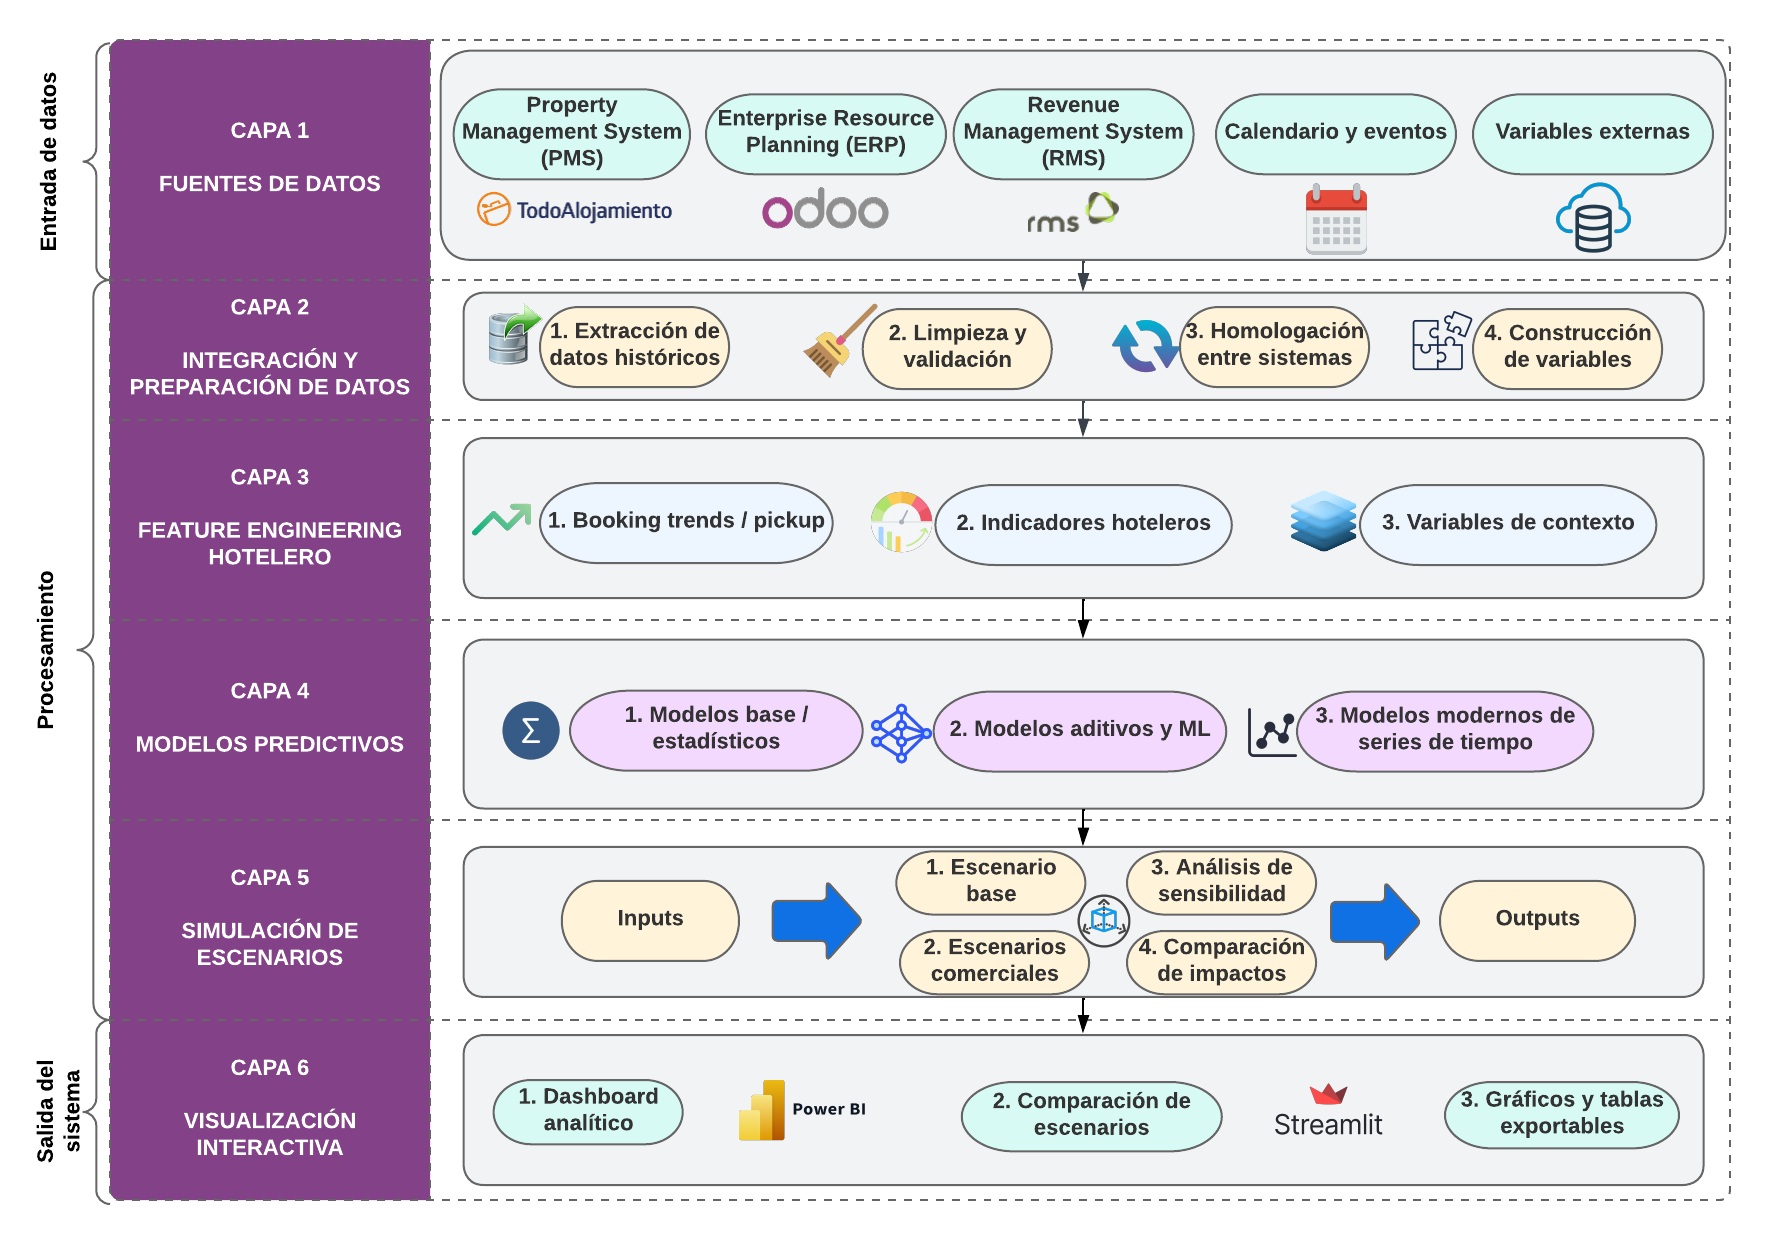
\includegraphics[width=.95\textwidth]{./Figuras/Diagrama_proyecto.png}
\caption{\centering Diagrama en bloques del sistema. El sistema integra datos operativos de los hoteles con modelos predictivos y simulación de escenarios, para apoyar la toma de decisiones comerciales.}
\label{fig:Diagrama_proyecto}
\end{figure}
\vspace{15px}
\pagebreak


\section{2. Identificación y análisis de los interesados}
\label{sec:interesados}


\begin{table}[ht]
%\caption{Identificación de los interesados}
%\label{tab:interesados}
\begin{tabularx}{\linewidth}{@{}|l|X|X|X|@{}}
\hline
\rowcolor[HTML]{C0C0C0} 
Rol           & Nombre y Apellido & Organización 	& Puesto 	\\ \hline
Cliente       & \clientename      &	\empclientename 	&	Gerente General, División Turismo       	\\ \hline
Responsable   & \authorname        & FIUBA        	& Alumno. 	\\ \hline
Orientador    & \supname	      & \pertesupname 	& Director del Trabajo Final \\ \hline
Colaboradores & Guillermo Alejandro \newline Francisco Lopez Ballent          & \empclientename             	& Referente comercial funcional \newline Líder de Proyectos y Excelencia Operativa \\ \hline
Usuario final & Equipo de Revenue Management / Comercial                 & \empclientename             	&  -      	\\ \hline
\end{tabularx}
\end{table}


A continuación, se listan las principales características de cada interesado:
\begin{itemize}
	\item Cliente: \clientename, como Gerente General de la División Turismo, es el principal responsable de aprobar los resultados del proyecto y colaborará en la definición del alcance y la validación de los entregables desde una mirada de negocio. El cliente requiere información confiable y anticipada para respaldar las decisiones comerciales y tarifarias de los tres hoteles de Tandil.
	\item Colaboradores: Guillermo Alejandro es el referente comercial funcional de la división y aportará el conocimiento del proceso actual de \textit{Revenue Management}, la interpretación de indicadores comerciales y la validación de los escenarios simulados. Francisco Lopez Ballent es el antecedente técnico interno del proyecto: líder del área de Proyectos y Excelencia Operativa, desarrolló previamente un pipeline de datos con información de reservas del sistema Arion (sistema PMS anterior 2022–2024) y realizó una prueba de concepto con modelos de proyección de demanda (Random Forest, XGBoost, LightGBM, Prophet), aunque no llegó a implementarse, ya que quedó en la etapa de diseño, luego de que las prioridades del negocio apuntaran al cambio completo de sistemas PMS, ERP y RMS.
	\item Orientador: el Ing. Joel Alexander Spak es Ingeniero Eléctrico, graduado de la Especialización en Inteligencia Artificial (FIUBA). En base a su experiencia, su Trabajo Final y a dos trabajos que luego dirigió, se demuestra su experiencia en las temáticas de proyección de series de tiempo.
	\item Usuario final: el equipo de \textit{Revenue Management} y Comercial de la División Turismo utilizará la herramienta como insumo en el proceso de planificación comercial y tarifaria de los hoteles de Tandil.
\end{itemize}


\section{3. Propósito del proyecto}
\label{sec:proposito}

El propósito de este proyecto es desarrollar una prueba de concepto de un sistema de soporte a decisiones para Revenue Management hotelero que proyecte demanda y ocupación esperada, analice el ritmo de reservas (\textit{booking pace}/\textit{pickup}) e incorpore un módulo de simulación de escenarios comerciales y tarifarios, integrando información histórica de reservas, ocupación y tarifas de los hoteles de Tandil de Grupo Faro Verde. La solución se encuentra en una etapa temprana del ciclo de vida: diseño conceptual,
relevamiento del proceso actual y planificación del desarrollo. Esta solución busca aportar una capa analítica complementaria al RMS recientemente incorporado por la organización, proporcionando información objetiva y anticipada que respalde la toma de decisiones comerciales de la División Turismo. Como diferencial adicional, y como alcance opcional, se buscará integrar los costos fijos y variables del ERP con el revenue proyectado, de modo de simular no solo el revenue esperado sino también el resultado económico de cada hotel frente al objetivo presupuestario anual con corte mensual.


\section{4. Alcance del proyecto}
\label{sec:alcance}

El proyecto se centrará en los tres hoteles de Tandil de Grupo Faro Verde (Mulen, La Cascada y Amaike), tomando como antecedente una prueba de concepto previa desarrollada internamente sobre datos de reservas del sistema Arion, que exploró modelos de proyección de demanda pero no llegó a implementarse. La innovación del proyecto radica en complementar el RMS recientemente incorporado con una capa analítica propia que integra proyección de demanda, análisis de \textit{pickup} y simulación de escenarios en una herramienta visual y accesible, retomando además una exploración técnica previa realizada dentro de la organización sobre datos de reservas, que no había llegado a implementarse. La solución permitirá analizar periódicamente la ocupación y el \textit{revenue} proyectado por hotel, junto con simulaciones de impacto ante cambios en tarifa promedio, mix de canales u otras variables comerciales, funcionando como insumo objetivo en el proceso de planificación comercial de la división.

Como diferencial adicional del proyecto, y sujeto a la disponibilidad y validación de datos, se evaluará la posibilidad de incorporar como alcance opcional la integración de los costos fijos y variables del ERP con la información de revenue proyectada. Esto permitiría extender la simulación de escenarios más allá del revenue esperado, proyectando también el resultado económico de cada hotel y comparándolo contra el objetivo presupuestario, definido con alcance anual y corte mensual, para cada uno de los hoteles de Tandil. De concretarse, este componente aportaría una mirada de rentabilidad y no solo comercial a la herramienta de soporte a decisiones.

El presente proyecto incluye:
\begin{itemize}
	\item El relevamiento funcional del proceso actual de \textit{Revenue Management} de la División Turismo, incluyendo el rol del RMS recientemente incorporado.
	\item La construcción de una base de datos analítica que integre información histórica de reservas, ocupación y tarifas, incorporando además variables de contexto referidas al calendario, eventos, clima y tipo de cambio.
	\item El diseño y validación de modelos de proyección de demanda y ocupación, evaluando modelos base y estadísticos (naive estacional, Holt-Winters/ETS, ARIMA/SARIMAX), modelos aditivos (Prophet) y modelos de \textit{machine learning} supervisado (Random Forest, XGBoost, LightGBM), y eventualmente algún enfoque moderno de series de tiempo.
	\item El análisis de indicadores de \textit{booking pace} o \textit{pickup} a distintos horizontes temporales, específicamente a los 1, 7, 14 o 30 días previos al check-in.
	\item El desarrollo de un módulo de simulación de escenarios comerciales/tarifarios, que permita comparar un escenario base contra alternativas modificando supuestos como tarifa promedio, ocupación esperada o mix de canales, y evaluar su impacto sobre indicadores como ocupación proyectada, ADR, RevPAR y revenue esperado.
	\item Una prueba de concepto visual, potencialmente en Streamlit, que permita explorar resultados, modificar supuestos y comparar escenarios.
	\item \textbf{(Opcional)} Como alcance opcional, se contempla la integración de los costos fijos y variables provenientes del ERP con la proyección de ingresos. El objetivo es simular no solo el ingreso esperado, sino también el resultado económico de cada hotel de Tandil, contrastándolo con el presupuesto anual de desglose mensual. La ejecución de este punto queda supeditada a la validación técnica de los datos de costos y al cumplimiento del cronograma principal del proyecto.
\end{itemize}


El presente proyecto no incluye:
\begin{itemize}
	\item El reemplazo o la integración productiva con el RMS ya incorporado por la organización.
	\item La automatización de la definición de tarifas ni la intervención en la configuración de los sistemas transaccionales (PMS, ERP, RMS).
	\item La incorporación de otros hoteles o unidades de negocio de Grupo Faro Verde fuera de los tres hoteles de Tandil.
	\item El entrenamiento formal a usuarios finales o su incorporación a la rutina operativa de la empresa.
\end{itemize}


\section{5. Supuestos del proyecto}
\label{sec:supuestos}

Para el desarrollo del presente proyecto se supone que:

\begin{itemize}
	\item Se contará con acceso oportuno a los \textit{datasets} históricos necesarios para el modelado (reservas, ocupación, tarifas, cancelaciones, calendario) provenientes del PMS, el ERP y el sistema Arion, en un formato utilizable y representativo de la operatoria real de los hoteles.
	\item Se asume el compromiso y la disponibilidad horaria del cliente y de los colaboradores funcionales y técnicos para participar en las sesiones de relevamiento, las revisiones de avance y la validación formal de los entregables.
	\item Se asume que la reciente actualización de sistemas (PMS, ERP y RMS) no impedirá reconstruir una base histórica homogénea, aunque pueda requerir tareas adicionales de integración y homologación entre períodos o sistemas.
	\item Se considera que las herramientas previstas (Python, bibliotecas de proyección y \textit{machine learning}, Streamlit) son adecuadas para el desarrollo de la prueba de concepto, y que no surgirán restricciones técnicas críticas que impidan ejecutar los modelos o visualizar los resultados.
	\item El proceso de desarrollo se llevará a cabo con el hardware y la conectividad del autor, empleando únicamente herramientas de código abierto para evitar la necesidad de inversiones extraordinarias en infraestructura o licencias de software.
	\item Se asume que no existirán bloqueos internos ni restricciones de confidencialidad que impidan el acceso a la información necesaria para el desarrollo y la validación de los modelos, más allá de los recaudos habituales de tratamiento de información comercial sensible.
	\item Para la interpretación de resultados y la simulación de escenarios, se asume que no ocurrirán cambios abruptos en el contexto macroeconómico (inflación, tipo de cambio, regulaciones turísticas) que invaliden los patrones históricos de demanda utilizados para el modelado.
	\item Se considera que los datos históricos disponibles reflejan adecuadamente la estacionalidad y variabilidad esperada de la demanda hotelera en Tandil, siendo válidos para el entrenamiento y evaluación de los modelos predictivos.
	\item Se asume la disponibilidad y adecuada granularidad de los datos de costos del ERP Odoo 18 para su integración con las proyecciones de \textit{revenue}. Del mismo modo, se considera que el acceso a los objetivos presupuestarios anuales con corte mensual de cada hotel está garantizado para su uso como parámetro de comparación.
\end{itemize}
\pagebreak

\section{6. Product Backlog}
\label{sec:backlog}

Los criterios para calcular los story points estarán divididos de la siguiente manera:
\begin{itemize}
	\item \textbf{Dificultad (1–13)}: evalúa el nivel de esfuerzo técnico y de desarrollo requerido.
	\item \textbf{Complejidad (1–13)}: referido al grado de conocimiento y experiencia necesarios.
	\item \textbf{Riesgo (1–13)}: pondera la incertidumbre técnica, la disponibilidad de datos o las dependencias externas (por ejemplo, de terceros dentro de la organización).
\end{itemize}

Para la ponderación en cada uno de ellos se utilizará la serie de Fibonacci desde el 1 al 13. La escala queda de la siguiente forma: muy bajo (1), bajo (3), medio (5), alto (8) y muy alto (13). El resultado de la suma de los tres criterios se aproxima al valor más cercano de la serie de Fibonacci (1, 2, 3, 5, 8, 13, 21, 34) para obtener el Story Point final de cada historia.

\subsection*{6.1. Épica 1: relevamiento e integración de datos hoteleros}
\begin{itemize}
  \item \textbf{Historia de usuario 1:} como Responsable de Análisis de Información, quiero relevar el proceso actual de Revenue Management de la División Turismo, para identificar qué información y decisiones debe soportar el sistema.
    \begin{itemize}
      \item \textbf{Dificultad}: bajo (3). Es un trabajo de relevamiento funcional, sin desarrollo técnico.
      \item \textbf{Complejidad}: bajo (3). Requiere coordinar reuniones y comprender el proceso de negocio y el rol del RMS.
      \item \textbf{Riesgo}: medio (5). Depende de la disponibilidad de tiempo de Diego y Guillermo.
      \item \textbf{Story Points} = 3 + 3 + 5 = 11 (se aproxima a 13).
      \item \textbf{Prioridad}: alta.
    \end{itemize}
  \item \textbf{Historia de usuario 2:} como analista de datos, quiero construir una base de datos analítica que integre reservas, ocupación y tarifas históricas de los tres hoteles, para contar con una fuente consolidada para el modelado.
    \begin{itemize}
      \item \textbf{Dificultad}: alto (8). Implica integrar el PMS, el ERP y el histórico del sistema Arion, con estructuras distintas.
      \item \textbf{Complejidad}: medio (5). Requiere homologar granularidad y formatos entre sistemas y períodos.
      \item \textbf{Riesgo}: medio (5). Riesgo de inconsistencias derivado del reciente cambio de sistemas.
      \item \textbf{Story Points} = 8 + 5 + 5 = 18 (se aproxima a 21).
      \item \textbf{Prioridad}: alta.
    \end{itemize}
  \item \textbf{Historia de usuario 3):} como analista de datos, quiero incorporar variables de contexto (calendario, eventos, clima, tipo de cambio) a la base analítica, para enriquecer el modelado de demanda.
    \begin{itemize}
      \item \textbf{Dificultad}: medio (5). Requiere identificar y obtener fuentes externas confiables.
      \item \textbf{Complejidad}: bajo (3). La integración en sí es de complejidad moderada.
      \item \textbf{Riesgo}: bajo (3). Depende de la disponibilidad de fuentes externas gratuitas.
      \item \textbf{Story Points} = 5 + 3 + 3 = 11 (se aproxima a 13).
      \item \textbf{Prioridad}: media.
    \end{itemize}
\end{itemize}

\subsection*{6.2. Épica 2: modelado predictivo de demanda y ocupación}
\begin{itemize}
  \item \textbf{Historia de usuario 4:} como responsable de Revenue Management, quiero contar con un modelo de proyección de demanda y ocupación por hotel, para anticipar la ocupación esperada en fechas futuras.
    \begin{itemize}
      \item \textbf{Dificultad}: alto (8). Requiere evaluar y comparar múltiples modelos (ARIMA/SARIMAX, Prophet, \textit{machine learning}).
      \item \textbf{Complejidad}: alto (8). Series con estacionalidad múltiple y datos heterogéneos entre hoteles.
      \item \textbf{Riesgo}: medio (5). Depende de la calidad y profundidad histórica de los datos.
      \item \textbf{Story Points} = 8 + 8 + 5 = 21.
      \item \textbf{Prioridad}: alta.
    \end{itemize}
  \item \textbf{Historia de usuario 5:} como analista comercial, quiero analizar indicadores de \textit{booking pace}/\textit{pickup} a distintos horizontes temporales (1, 7, 14 o 30 días antes del check-in), para entender el ritmo de reservas previo a la estadía.
    \begin{itemize}
      \item \textbf{Dificultad}: medio (5). Requiere construir variables de \textit{feature engineering} específicas.
      \item \textbf{Complejidad}: medio (5). Involucra el cruce de fecha de reserva y fecha de estadía.
      \item \textbf{Riesgo}: bajo (3). Depende de la trazabilidad histórica de fechas de reserva.
      \item \textbf{Story Points} = 5 + 5 + 3 = 13.
      \item \textbf{Prioridad}: alta.
    \end{itemize}
    \item \textbf{Historia de usuario 6:} como analista de datos, quiero comparar el desempeño de distintos modelos de proyección (estadísticos vs. \textit{machine learning}) en validación temporal, para seleccionar el enfoque más adecuado para cada hotel y que el responsable de Revenue Management cuente con proyecciones confiables.
    \begin{itemize}
      \item \textbf{Dificultad}: medio (5). Requiere definir y aplicar métricas de validación temporal.
      \item \textbf{Complejidad}: medio (5). Supone comparar resultados entre familias de modelos distintas.
      \item \textbf{Riesgo}: bajo (3). Bajo riesgo, dado que se trata de una etapa de evaluación.
      \item \textbf{Story Points} = 5 + 5 + 3 = 13.
      \item \textbf{Prioridad}: media.
    \end{itemize}
\end{itemize}

\subsection*{6.3. Épica 3: simulación de escenarios comerciales}
\begin{itemize}
  \item \textbf{Historia de usuario 7:} como responsable comercial, quiero simular escenarios modificando la tarifa promedio, la ocupación esperada o el mix de canales, para evaluar su impacto en la ocupación proyectada, el ADR, el RevPAR y el revenue esperado.
    \begin{itemize}
      \item \textbf{Dificultad}: alto (8). Requiere vincular los modelos predictivos con una capa de simulación paramétrica.
      \item \textbf{Complejidad}: medio (5). Debe considerar la sensibilidad conjunta de varias variables comerciales.
      \item \textbf{Riesgo}: bajo (3). El riesgo se acota a la calibración de los parámetros de simulación.
      \item \textbf{Story Points} = 8 + 5 + 3 = 16 (se aproxima a 13).
      \item \textbf{Prioridad}: alta.
    \end{itemize}
  \item \textbf{Historia de usuario 8:} como Gerente General de la División Turismo, quiero comparar un escenario base contra escenarios alternativos, para fundamentar decisiones tarifarias con datos objetivos.
    \begin{itemize}
      \item \textbf{Dificultad}: medio (5). Requiere definir la lógica de comparación entre escenarios.
      \item \textbf{Complejidad}: bajo (3). Es una funcionalidad que se apoya en el módulo de simulación ya construido.
      \item \textbf{Riesgo}: bajo (3). Bajo riesgo, dado que reutiliza los outputs de la HU7.
      \item \textbf{Story Points} = 5 + 3 + 3 = 11 (se aproxima a 13).
      \item \textbf{Prioridad}: alta.
    \end{itemize}
  \item \textbf{Historia de usuario 9 (opcional):} como responsable de control de gestión, quiero integrar los costos fijos y variables del ERP al revenue proyectado, para simular el resultado económico de cada hotel frente al presupuesto anual con corte mensual.
    \begin{itemize}
      \item \textbf{Dificultad}: alto (8). Requiere modelar la estructura de costos por hotel y por mes.
      \item \textbf{Complejidad}: medio (5). Implica combinar dos fuentes de información de naturaleza distinta (ingresos proyectados y costos reales).
      \item \textbf{Riesgo}: alto (8). Depende fuertemente de la disponibilidad y granularidad de los datos de costos en el ERP.
      \item \textbf{Story Points} = 8 + 5 + 8 = 21.
      \item \textbf{Prioridad}: baja (opcional).
    \end{itemize}
\end{itemize}

\subsection*{6.4. Épica 4: visualización y prueba de concepto (PoC)}
\begin{itemize}
  \item \textbf{Historia de usuario 10:} como usuario final del equipo de \textit{Revenue Management}, quiero visualizar en un \textit{dashboard} interactivo la ocupación y el revenue proyectado por hotel, para monitorear los indicadores clave del negocio.
    \begin{itemize}
      \item \textbf{Dificultad}: medio (5). Requiere conectar los resultados de los modelos con la interfaz de visualización.
      \item \textbf{Complejidad}: bajo (3). Se apoya en herramientas estándar como Streamlit.
      \item \textbf{Riesgo}: bajo (3). Bajo riesgo si los datos ya están procesados en etapas anteriores.
      \item \textbf{Story Points} = 5 + 3 + 3 = 11 (se aproxima a 13).
      \item \textbf{Prioridad}: alta.
    \end{itemize}
  \item \textbf{Historia de usuario 11:} como responsable comercial, quiero filtrar y comparar escenarios (base vs. alternativo) desde la misma interfaz, para agilizar la toma de decisiones sin depender de reportes externos.
    \begin{itemize}
      \item \textbf{Dificultad}: bajo (3). Es una funcionalidad de filtrado y comparación visual.
      \item \textbf{Complejidad}: bajo (3). Requiere lógica de selección entre escenarios ya calculados.
      \item \textbf{Riesgo}: muy bajo (1). Bajo riesgo, ya que los datos subyacentes ya están validados.
      \item \textbf{Story Points} = 3 + 3 + 1 = 7 (se aproxima a 8).
      \item \textbf{Prioridad}: media.
    \end{itemize}
  \item \textbf{Historia de usuario 12 (opcional):} como usuario final, quiero exportar los gráficos y tablas de resultados, para incluirlos en reportes internos de la división.
    \begin{itemize}
      \item \textbf{Dificultad}: bajo (2). Es una funcionalidad estándar de exportación.
      \item \textbf{Complejidad}: muy bajo (1). Muy baja, al reutilizar componentes ya disponibles en la herramienta de visualización.
      \item \textbf{Riesgo}: nulo (0). Prácticamente nulo.
      \item \textbf{Story Points} = 2 + 1 + 0 = 3.
      \item \textbf{Prioridad}: baja.
    \end{itemize}
\end{itemize}


\section{7. Criterios de aceptación de historias de usuario}
\label{sec:criteriosAceptacion}

En esta sección se definen los criterios de aceptación para cada historia de usuario del \textit{backlog}, con el objetivo de establecer condiciones específicas, medibles y verificables que permitan validar la funcionalidad desarrollada.

Se utiliza el modelo Gherkin, un enfoque ampliamente adoptado en metodologías ágiles para describir escenarios de prueba funcional en lenguaje natural estructurado. Este modelo sigue una sintaxis sencilla basada en las siguientes expresiones clave:

\begin{itemize}
  \item \textbf{Dado (Given)}: establece el contexto inicial o condiciones previas.
  \item \textbf{Cuando (When)}: describe la acción que se va a realizar.
  \item \textbf{Entonces (Then)}: indica el resultado esperado que permite validar el cumplimiento de la funcionalidad.
\end{itemize}

Este formato permite una comprensión clara tanto por parte de usuarios técnicos como no técnicos, facilitando la colaboración y alineamiento entre el alumno, el cliente y los colaboradores del proyecto.

\subsection*{7.1. Épica 1: relevamiento e integración de datos hoteleros}

\paragraph{Criterios de aceptación HU1: relevamiento del proceso actual de Revenue Management}
\begin{itemize}
  \item \textbf{Criterio 1} \\
  \textbf{Dado} el acceso a los referentes comercial y técnico de la División Turismo, \\
  \textbf{cuando} se realicen las sesiones de relevamiento funcional, \\
  \textbf{entonces} debe quedar documentado el proceso actual de \textit{Revenue Management}, incluyendo el rol del RMS y los principales puntos de decisión comercial.

  \item \textbf{Criterio 2} \\
  \textbf{Dado} el relevamiento realizado, \\
  \textbf{cuando} se identifiquen las necesidades de información del cliente, \\
  \textbf{entonces} debe existir un documento de requerimientos validado por \clientename.

  \item \textbf{Criterio 3} \\
  \textbf{Dado} el proceso relevado, \\
  \textbf{cuando} se lo contraste con el alcance definido del proyecto, \\
  \textbf{entonces} deben quedar explícitamente identificadas las brechas de información que el sistema propuesto busca cubrir.
\end{itemize}

\vspace{1em}

\paragraph{Criterios de aceptación HU2: construcción de la base de datos analítica}
\begin{itemize}
  \item \textbf{Criterio 1} \\
  \textbf{Dado} el acceso a los datos históricos del PMS, el ERP y el sistema Arion, \\
  \textbf{cuando} se ejecute el proceso de extracción e integración, \\
  \textbf{entonces} debe generarse una base analítica única con reservas, ocupación y tarifas homologadas entre sistemas.

  \item \textbf{Criterio 2} \\
  \textbf{Dado} un período histórico determinado, \\
  \textbf{cuando} se valide la granularidad de los datos integrados, \\
  \textbf{entonces} la base debe mantener una granularidad diaria consistente para todos los hoteles y períodos disponibles.

  \item \textbf{Criterio 3} \\
  \textbf{Dado} la base de datos construida, \\
  \textbf{cuando} se realicen controles de calidad, \\
  \textbf{entonces} no deben existir registros duplicados ni inconsistencias entre fecha de reserva, fecha de check-in y fecha de check-out.
\end{itemize}

\vspace{1em}

\paragraph{Criterios de aceptación HU3: incorporación de variables de contexto}
\begin{itemize}
  \item \textbf{Criterio 1} \\
  \textbf{Dado} un calendario de feriados y eventos locales de Tandil, \\
  \textbf{cuando} se lo incorpore a la base analítica, \\
  \textbf{entonces} cada fecha debe quedar etiquetada según corresponda a día de semana, fin de semana largo o evento especial.

  \item \textbf{Criterio 2} \\
  \textbf{Dado} una fuente externa de tipo de cambio, \\
  \textbf{cuando} se integre a la base analítica, \\
  \textbf{entonces} cada registro histórico debe contar con el valor de tipo de cambio correspondiente a su fecha.

  \item \textbf{Criterio 3} \\
  \textbf{Dado} las variables de contexto incorporadas, \\
  \textbf{cuando} se utilicen como \textit{input} de los modelos predictivos, \\
  \textbf{entonces} no deben generarse valores faltantes no controlados para el período de entrenamiento.
\end{itemize}

\subsection*{7.2. Épica 2: modelado predictivo de demanda y ocupación}

\paragraph{Criterios de aceptación HU4: modelo de proyección de demanda y ocupación por hotel}
\begin{itemize}
  \item \textbf{Criterio 1} \\
  \textbf{Dado} un conjunto de datos históricos de ocupación por hotel, \\
  \textbf{cuando} se entrene el modelo seleccionado, \\
  \textbf{entonces} debe generarse una proyección de ocupación diaria para al menos los siguientes 30 días, para cada uno de los tres hoteles.

  \item \textbf{Criterio 2} \\
  \textbf{Dado} un conjunto de datos de validación temporal (\textit{holdout}), \\
  \textbf{cuando} se evalúe el modelo entrenado, \\
  \textbf{entonces} el error de proyección (por ejemplo, MAPE) debe quedar documentado y ser inferior al umbral definido como aceptable para el proyecto.

  \item \textbf{Criterio 3} \\
  \textbf{Dado} el modelo de demanda y ocupación, \\
  \textbf{cuando} se calculen los indicadores derivados, \\
  \textbf{entonces} debe poder obtenerse automáticamente el ADR y el RevPAR proyectados por hotel.
\end{itemize}

\vspace{1em}

\paragraph{Criterios de aceptación HU5: indicadores de booking pace/pickup}
\begin{itemize}
  \item \textbf{Criterio 1} \\
  \textbf{Dado} una fecha de estadía futura, \\
  \textbf{cuando} se consulten las reservas \textit{on the books}, \\
  \textbf{entonces} debe poder obtenerse la cantidad de reservas acumuladas a 1, 7, 14 y 30 días antes del check-in.

  \item \textbf{Criterio 2} \\
  \textbf{Dado} dos horizontes temporales consecutivos (por ejemplo, 14 y 7 días antes del check-in), \\
  \textbf{cuando} se calcule el \textit{pickup}, \\
  \textbf{entonces} debe obtenerse la variación de reservas entre ambos horizontes, por hotel y por fecha de estadía.

  \item \textbf{Criterio 3} \\
  \textbf{Dado} el histórico de \textit{booking pace} calculado, \\
  \textbf{cuando} se lo compare contra fechas análogas de temporadas anteriores, \\
  \textbf{entonces} debe poder identificarse si el ritmo de reservas actual está por encima o por debajo del patrón histórico.
\end{itemize}

\vspace{1em}

\paragraph{Criterios de aceptación HU6: comparación de modelos de proyección}
\begin{itemize}
  \item \textbf{Criterio 1} \\
  \textbf{Dado} un conjunto de modelos candidatos (estadísticos y de \textit{machine learning}), \\
  \textbf{cuando} se evalúen sobre el mismo conjunto de validación temporal, \\
  \textbf{entonces} debe generarse una tabla comparativa de métricas de error por modelo y por hotel.

  \item \textbf{Criterio 2} \\
  \textbf{Dado} los resultados de la comparación, \\
  \textbf{cuando} se seleccione el modelo final para cada hotel, \\
  \textbf{entonces} la elección debe quedar justificada en función de precisión, robustez e interpretabilidad.

  \item \textbf{Criterio 3} \\
  \textbf{Dado} el modelo seleccionado, \\
  \textbf{cuando} se lo documente en la memoria del proyecto, \\
  \textbf{entonces} deben quedar registrados los hiperparámetros y el criterio de selección utilizados.
\end{itemize}

\subsection*{7.3. Épica 3: simulación de escenarios comerciales}

\paragraph{Criterios de aceptación HU7: simulación de escenarios comerciales/tarifarios}
\begin{itemize}
  \item \textbf{Criterio 1} \\
  \textbf{Dado} un escenario definido por el usuario (tarifa promedio, ocupación esperada o mix de canales), \\
  \textbf{cuando} se ejecute la simulación, \\
  \textbf{entonces} deben recalcularse la ocupación proyectada, el ADR, el RevPAR y el revenue esperado para dicho escenario.

  \item \textbf{Criterio 2} \\
  \textbf{Dado} un rango de valores posibles para una variable comercial (por ejemplo, tarifa promedio), \\
  \textbf{cuando} se realice un análisis de sensibilidad, \\
  \textbf{entonces} debe mostrarse cómo varía el revenue esperado ante cada valor del rango.

  \item \textbf{Criterio 3} \\
  \textbf{Dado} un escenario simulado, \\
  \textbf{cuando} se modifiquen sus supuestos, \\
  \textbf{entonces} los resultados deben actualizarse sin necesidad de volver a entrenar los modelos predictivos de base.
\end{itemize}

\vspace{1em}

\paragraph{Criterios de aceptación HU8: comparación de escenario base vs. alternativo}
\begin{itemize}
  \item \textbf{Criterio 1} \\
  \textbf{Dado} un escenario base y al menos un escenario alternativo, \\
  \textbf{cuando} se comparen ambos, \\
  \textbf{entonces} debe mostrarse la diferencia absoluta y porcentual en ocupación, ADR, RevPAR y revenue esperado.

  \item \textbf{Criterio 2} \\
  \textbf{Dado} más de un escenario alternativo simulado, \\
  \textbf{cuando} se los ordene por resultado, \\
  \textbf{entonces} debe poder identificarse cuál maximiza el revenue esperado para cada hotel.

  \item \textbf{Criterio 3} \\
  \textbf{Dado} la comparación de escenarios, \\
  \textbf{cuando} \clientename\hspace{1px} la revise, \\
  \textbf{entonces} debe poder utilizarla como insumo objetivo para una decisión comercial concreta.
\end{itemize}

\vspace{1em}

\paragraph{Criterios de aceptación HU9 (opcional): integración de costos ERP y resultado económico}
\begin{itemize}
  \item \textbf{Criterio 1} \\
  \textbf{Dado} los costos fijos y variables disponibles en el ERP (Odoo 18) para un hotel y un mes determinado, \\
  \textbf{cuando} se los integre con el revenue proyectado, \\
  \textbf{entonces} debe calcularse el resultado económico proyectado de ese hotel para ese mes.

  \item \textbf{Criterio 2} \\
  \textbf{Dado} el resultado económico proyectado, \\
  \textbf{cuando} se lo compare contra el objetivo presupuestario anual con corte mensual, \\
  \textbf{entonces} debe mostrarse el desvío absoluto y porcentual respecto al presupuesto de cada hotel.

  \item \textbf{Criterio 3} \\
  \textbf{Dado} que la información de costos del ERP no esté disponible con el detalle necesario, \\
  \textbf{cuando} se intente ejecutar esta funcionalidad, \\
  \textbf{entonces} el sistema debe informar la limitación en lugar de mostrar un resultado económico no validado.
\end{itemize}

\subsection*{7.4. Épica 4: visualización y prueba de concepto (PoC)}

\paragraph{Criterios de aceptación HU10: dashboard de ocupación y revenue proyectado}
\begin{itemize}
  \item \textbf{Criterio 1} \\
  \textbf{Dado} los resultados de los modelos predictivos, \\
  \textbf{cuando} se acceda al \textit{dashboard}, \\
  \textbf{entonces} deben visualizarse la ocupación y el revenue proyectado por hotel, con filtros por fecha, hotel, canal y segmento.

  \item \textbf{Criterio 2} \\
  \textbf{Dado} un hotel seleccionado en el \textit{dashboard}, \\
  \textbf{cuando} el usuario cambie de hotel, \\
  \textbf{entonces} todos los indicadores mostrados deben actualizarse en consecuencia.

  \item \textbf{Criterio 3} \\
  \textbf{Dado} el \textit{dashboard} en funcionamiento, \\
  \textbf{cuando} lo utilice un usuario del equipo de \textit{Revenue Management} sin conocimientos técnicos, \\
  \textbf{entonces} debe poder interpretar los indicadores principales sin asistencia del alumno.
\end{itemize}

\vspace{1em}

\paragraph{Criterios de aceptación HU11: comparación de escenarios desde la interfaz}
\begin{itemize}
  \item \textbf{Criterio 1} \\
  \textbf{Dado} un escenario base y un escenario alternativo ya simulados, \\
  \textbf{cuando} el usuario los seleccione desde la interfaz, \\
  \textbf{entonces} deben visualizarse ambos de forma comparativa en un mismo gráfico o tabla.

  \item \textbf{Criterio 2} \\
  \textbf{Dado} varios escenarios alternativos disponibles, \\
  \textbf{cuando} el usuario aplique un filtro de comparación, \\
  \textbf{entonces} solo deben mostrarse los escenarios seleccionados, sin necesidad de recalcular resultados.

  \item \textbf{Criterio 3} \\
  \textbf{Dado} la comparación visualizada, \\
  \textbf{cuando} el usuario cambie de escenario alternativo, \\
  \textbf{entonces} el tiempo de respuesta de la interfaz debe ser adecuado para su uso en una reunión comercial.
\end{itemize}

\vspace{1em}

\paragraph{Criterios de aceptación HU12 (opcional): exportación de gráficos y tablas}
\begin{itemize}
  \item \textbf{Criterio 1} \\
  \textbf{Dado} un gráfico o tabla de resultados generado en el \textit{dashboard}, \\
  \textbf{cuando} el usuario solicite exportarlo, \\
  \textbf{entonces} debe poder descargarse en un formato estándar (por ejemplo, PNG, CSV o Excel).

  \item \textbf{Criterio 2} \\
  \textbf{Dado} un reporte exportado, \\
  \textbf{cuando} se lo abra fuera de la herramienta de visualización, \\
  \textbf{entonces} debe conservar los datos y etiquetas necesarios para su interpretación sin depender del sistema original.

  \item \textbf{Criterio 3} \\
  \textbf{Dado} que esta funcionalidad no llegue a implementarse por restricciones de tiempo, \\
  \textbf{cuando} se documente el cierre del proyecto, \\
  \textbf{entonces} debe quedar explícitamente señalada como alcance opcional no concretado, sin afectar el resto de los entregables.
\end{itemize}

\section{8. Fases de CRISP-DM}

\subsection*{8.1. Comprensión del negocio}
El objetivo del proyecto es aportar una capa analítica complementaria al proceso de \textit{Revenue Management} de la División Turismo de Grupo Faro Verde, mediante un sistema que permita proyectar demanda y ocupación, analizar el ritmo de reservas (\textit{booking pace}) y simular escenarios comerciales y tarifarios para los hoteles de Tandil. El valor agregado de la inteligencia artificial radica en reemplazar el análisis puramente manual e histórico por proyecciones objetivas basadas en datos, que permitan anticipar decisiones en lugar de reaccionar sobre resultados ya ocurridos. El éxito del proyecto será evaluado mediante la precisión de los modelos de proyección, la utilidad percibida de las simulaciones de escenarios por parte del cliente y los colaboradores, y la adopción efectiva de la herramienta como insumo en el proceso de planificación comercial.

\subsection*{8.2. Comprensión de los datos}
Los datos provienen principalmente del sistema Arion (histórico de reservas 2022-2024), del \textit{Property Management System} actualmente en uso (PMS, Todo Alojamiento) y del ERP (Odoo 18 Community), con información de reservas, ocupación, tarifas, cancelaciones e ingresos por hotel. Se cuenta con registros históricos con una profundidad razonable, aunque la reciente migración de sistemas (PMS, ERP y RMS) introduce desafíos de calidad, como posibles diferencias de granularidad, codificación o cobertura temporal entre el sistema anterior y el actual. Parte de esta etapa consiste en relevar y documentar estas diferencias antes de avanzar a la preparación de los datos.

\subsection*{8.3. Preparación de los datos}
Durante esta fase se realizará la limpieza, homologación e integración de los datos, lo cual incluye:
\begin{itemize}
  \item Extracción y consolidación de los datos históricos de reservas, ocupación y tarifas provenientes del PMS, el ERP y el sistema Arion.
  \item Homologación de estructuras y granularidad entre sistemas y períodos, dado el reciente cambio tecnológico de la división.
  \item Tratamiento de valores faltantes, cancelaciones y registros inconsistentes.
  \item Construcción de variables de \textit{feature engineering} hotelero: variables temporales (día de semana, temporada, feriados), indicadores de \textit{booking pace}/\textit{pickup} (1, 7, 14 y 30 días antes del check-in) e indicadores hoteleros (ADR, RevPAR).
  \item Incorporación de variables de contexto externas (calendario de eventos, clima, tipo de cambio).
\end{itemize}
La preparación de los datos resulta crítica en este proyecto, dado que la calidad y consistencia de la base analítica condicionan directamente la confiabilidad de los modelos de proyección y de la simulación de escenarios.

\subsection*{8.4. Modelado}
El problema principal es de predicción de series de tiempo (demanda y ocupación diaria por hotel), complementado con un módulo de simulación de escenarios comerciales. Se evaluarán modelos de distinta naturaleza:
\begin{itemize}
  \item Modelos base y estadísticos: naive estacional, Holt-Winters/ETS y ARIMA/SARIMAX, para capturar tendencia y estacionalidad.
  \item Modelos aditivos: Prophet, para incorporar de forma explícita feriados, eventos y múltiples estacionalidades.
  \item Modelos de \textit{machine learning} supervisado: Random Forest, XGBoost y LightGBM, para incorporar variables de contexto y de \textit{booking pace} como predictoras.
  \item Eventualmente, algún enfoque moderno de series de tiempo (por ejemplo, N-BEATS o TFT), si la profundidad y calidad de los datos lo permiten.
\end{itemize}
Sobre los modelos seleccionados se construirá, además, la capa de simulación de escenarios comerciales/tarifarios descripta en el Alcance del proyecto.

\subsection*{8.5. Evaluación del modelo}
Los modelos de proyección se evaluarán mediante métricas clásicas de error en validación temporal (\textit{backtesting}), tales como:
\begin{itemize}
  \item MAE (\textit{Mean Absolute Error}) y MAPE (\textit{Mean Absolute Percentage Error}) para la proyección de ocupación y demanda.
  \item RMSE (\textit{Root Mean Squared Error}), para penalizar errores de mayor magnitud.
  \item Comparación del desempeño entre modelos candidatos por hotel, priorizando aquellos que combinen precisión, robustez e interpretabilidad (indicado en la HU6).
\end{itemize}
Adicionalmente, el módulo de simulación de escenarios se evaluará de forma cualitativa junto con el cliente y los colaboradores, verificando que los resultados frente a cambios de tarifa, ocupación o mix de canales resulten razonables y útiles para la toma de decisiones.

\subsection*{8.6. Despliegue del modelo (opcional)}
El sistema se implementará como una prueba de concepto (PoC), mediante una visualización interactiva potencialmente desarrollada en Streamlit. En esta instancia, la herramienta funcionará como un tablero de uso interno para el equipo de \textit{Revenue Management} y Comercial de la División Turismo, con capacidad de explorar proyecciones y simular escenarios comerciales. No se prevé integración productiva con el PMS, el ERP ni el RMS durante esta etapa, aunque sí se documentarán recomendaciones para una eventual evolución hacia un despliegue productivo.

\section{9. Desglose del trabajo en tareas}
\label{sec:wbs}
 
A partir de cada Historia de Usuario (HU) definida en la sección 6, se descompone el trabajo en tareas técnicas concretas, medibles y acotadas en el tiempo, indicando su estimación en horas hombre y su prioridad relativa (Alta, Media o Baja). La estimación de cada tarea guarda coherencia con los \textit{Story Points} asignados en el \textit{Product Backlog}: las HU de mayor tamaño relativo (por ejemplo, HU2, HU4 y HU9) concentran una mayor cantidad de horas y de tareas, mientras que las de menor tamaño (por ejemplo, HU11 y HU12) requieren un desglose más acotado. El esfuerzo total estimado para el desarrollo del proyecto (incluyendo la planificación previa y la documentación final) asciende a 648 horas, distribuido de forma equilibrada entre las cuatro épicas.

\subsection*{9.0. Planificación del proyecto (previo al desarrollo)}
 
\begin{table}[H]
\centering
\begin{tabularx}{\linewidth}{@{}|X|X|c|c|@{}}
\hline
\rowcolor[HTML]{C0C0C0}
Historia de usuario & Tarea técnica & Estimación & Prioridad \\ \hline
N/A & Reunión inicial con el cliente y recolección de requerimientos & 3 h & Alta \\ \hline
N/A & Lectura de documentos de contexto del negocio (Grupo Faro Verde, hoteles de Tandil) & 2 h & Alta \\ \hline
N/A & Validación de problemas con \textit{stakeholders} (Diego, Guillermo, Francisco) & 3 h & Alta \\ \hline
N/A & Revisión de lineamientos académicos para el plan de proyecto & 3 h & Alta \\ \hline
N/A & Búsqueda y contacto de potenciales directores & 2 h & Media \\ \hline
N/A & Coordinación de reunión para validación del tema con el director & 2 h & Media \\ \hline
N/A & Redacción inicial del documento de planificación (secciones 1 a 5) & 6 h & Alta \\ \hline
N/A & Elaboración del cronograma preliminar y entregables & 3 h & Alta \\ \hline
N/A & Ajuste del documento según \textit{feedback} de la primera entrega & 3 h & Alta \\ \hline
N/A & Preparación y entrega formal del plan (versión final) & 4 h & Alta \\ \hline
\end{tabularx}
\caption{Desglose de tareas para la planificación del proyecto.}
\end{table}
  
%\vspace{0.5cm}
\noindent
\textbf{Total estimado parcial:} \textbf{31 horas.}

\subsection*{9.1. Épica 1: relevamiento e integración de datos hoteleros}
 
\begin{table}[H]
\centering
\begin{tabularx}{\linewidth}{@{}|X|X|c|c|@{}}
\hline
\rowcolor[HTML]{C0C0C0}
Historia de usuario & Tarea técnica & Estimación & Prioridad \\ \hline
HU1 & Coordinación de sesiones de relevamiento con Diego y Guillermo & 4 h & Alta \\ \hline
HU1 & Relevamiento funcional del proceso actual de \textit{Revenue Management} & 8 h & Alta \\ \hline
HU1 & Relevamiento del rol y alcance del RMS recientemente incorporado & 6 h & Alta \\ \hline
HU1 & Análisis de los principales puntos de decisión comercial actuales & 6 h & Alta \\ \hline
HU1 & Documentación del proceso relevado & 6 h & Alta \\ \hline
HU1 & Validación del relevamiento con el cliente & 5 h & Alta \\ \hline
HU1 & Identificación de brechas de información a cubrir & 6 h & Media \\ \hline
HU1 & Ajustes al relevamiento según \textit{feedback} del cliente & 5 h & Media \\ \hline
\end{tabularx}
\caption{Desglose de tareas para HU1 (Épica 1: relevamiento e integración de datos hoteleros).}
\end{table}
 
\begin{table}[H]
\centering
\begin{tabularx}{\linewidth}{@{}|X|X|c|c|@{}}
\hline
\rowcolor[HTML]{C0C0C0}
Historia de usuario & Tarea técnica & Estimación & Prioridad \\ \hline
HU2 & Extracción de datos históricos del sistema Arion & 8 h & Alta \\ \hline
HU2 & Extracción de datos del PMS (Todo Alojamiento) & 8 h & Alta \\ \hline
HU2 & Extracción de datos de ingresos y costos del ERP (Odoo 18) & 6 h & Alta \\ \hline
HU2 & Diseño del esquema de la base de datos analítica & 6 h & Alta \\ \hline
HU2 & Homologación de estructuras entre sistemas y períodos & 10 h & Alta \\ \hline
HU2 & Ajuste de granularidad histórica entre fuentes & 8 h & Alta \\ \hline
HU2 & Limpieza de datos y tratamiento de duplicados/inconsistencias & 9 h & Alta \\ \hline
HU2 & Controles de calidad sobre fechas de reserva/check-in/check-out & 7 h & Alta \\ \hline
HU2 & Validación de la base construida con datos de muestra & 6 h & Alta \\ \hline
HU2 & Documentación técnica de la base analítica & 6 h & Media \\ \hline
\end{tabularx}
\caption{Desglose de tareas para HU2 (Épica 1: relevamiento e integración de datos hoteleros).}
\end{table}
 
\begin{table}[H]
\centering
\begin{tabularx}{\linewidth}{@{}|X|X|c|c|@{}}
\hline
\rowcolor[HTML]{C0C0C0}
Historia de usuario & Tarea técnica & Estimación & Prioridad \\ \hline
HU3 & Relevamiento de fuentes externas disponibles (calendario, clima, tipo de cambio) & 6 h & Media \\ \hline
HU3 & Extracción del calendario de feriados y eventos de Tandil & 6 h & Media \\ \hline
HU3 & Extracción de series históricas de tipo de cambio & 6 h & Media \\ \hline
HU3 & Extracción de datos climáticos históricos & 6 h & Media \\ \hline
HU3 & Integración de las variables de contexto a la base analítica & 10 h & Media \\ \hline
HU3 & Validación de cobertura y calidad de las variables incorporadas & 7 h & Media \\ \hline
HU3 & Documentación de las fuentes externas utilizadas & 5 h & Media \\ \hline
\end{tabularx}
\caption{Desglose de tareas para HU3 (Épica 1: relevamiento e integración de datos hoteleros).}
\end{table}
 
%\vspace{0.5cm}
\noindent
\textbf{Total estimado parcial:} \textbf{166 horas.}

\subsection*{9.2. Épica 2: modelado predictivo de demanda y ocupación}
 
\begin{table}[H]
\centering
\begin{tabularx}{\linewidth}{@{}|X|X|c|c|@{}}
\hline
\rowcolor[HTML]{C0C0C0}
Historia de usuario & Tarea técnica & Estimación & Prioridad \\ \hline
HU4 & Análisis exploratorio de series históricas por hotel & 7 h & Alta \\ \hline
HU4 & Implementación de modelos base (naive estacional, Holt-Winters/ETS) & 6 h & Alta \\ \hline
HU4 & Implementación de modelos ARIMA/SARIMAX & 9 h & Alta \\ \hline
HU4 & Implementación de modelo Prophet & 8 h & Alta \\ \hline
HU4 & Ajuste de hiperparámetros y estacionalidades múltiples & 9 h & Alta \\ \hline
HU4 & Entrenamiento de modelos de \textit{machine learning} (RF, XGBoost, LightGBM) & 9 h & Alta \\ \hline
HU4 & Validación cruzada temporal (\textit{backtesting}) por hotel & 8 h & Alta \\ \hline
HU4 & Cálculo de ADR y RevPAR proyectados & 6 h & Alta \\ \hline
HU4 & Documentación técnica del modelo seleccionado por hotel & 6 h & Media \\ \hline
HU4 & Ajustes finales según revisión con el orientador & 6 h & Media \\ \hline
\end{tabularx}
\caption{Desglose de tareas para HU4 (Épica 2: modelado predictivo de demanda y ocupación).}
\end{table}
 
\begin{table}[H]
\centering
\begin{tabularx}{\linewidth}{@{}|X|X|c|c|@{}}
\hline
\rowcolor[HTML]{C0C0C0}
Historia de usuario & Tarea técnica & Estimación & Prioridad \\ \hline
HU5 & Diseño de variables de \textit{booking pace} a distintos horizontes (1, 7, 14 y 30 días) & 7 h & Alta \\ \hline
HU5 & Implementación del cálculo de reservas \textit{on the books} & 8 h & Alta \\ \hline
HU5 & Cálculo de \textit{pickup} entre horizontes consecutivos & 8 h & Alta \\ \hline
HU5 & Comparación de \textit{booking pace} actual vs. patrones históricos & 8 h & Alta \\ \hline
HU5 & Visualización preliminar de indicadores de \textit{booking pace} & 7 h & Media \\ \hline
HU5 & Documentación de los indicadores de \textit{booking pace} & 8 h & Media \\ \hline
\end{tabularx}
\caption{Desglose de tareas para HU5 (Épica 2: modelado predictivo de demanda y ocupación).}
\end{table}
 
\begin{table}[H]
\centering
\begin{tabularx}{\linewidth}{@{}|X|X|c|c|@{}}
\hline
\rowcolor[HTML]{C0C0C0}
Historia de usuario & Tarea técnica & Estimación & Prioridad \\ \hline
HU6 & Diseño del esquema de validación temporal comparativo & 6 h & Media \\ \hline
HU6 & Ejecución comparativa de modelos estadísticos vs. ML por hotel & 10 h & Alta \\ \hline
HU6 & Cálculo y análisis de métricas de error (MAE, MAPE, RMSE) & 8 h & Alta \\ \hline
HU6 & Selección y justificación del modelo final por hotel & 8 h & Media \\ \hline
HU6 & Documentación de hiperparámetros y criterio de selección & 7 h & Media \\ \hline
HU6 & Presentación de resultados de la comparación al orientador & 7 h & Media \\ \hline
\end{tabularx}
\caption{Desglose de tareas para HU6 (Épica 2: modelado predictivo de demanda y ocupación).}
\end{table}
 
%\vspace{0.5cm}
\noindent
\textbf{Total estimado parcial:} \textbf{166 horas.}
 
\subsection*{9.3. Épica 3: simulación de escenarios comerciales}
 
\begin{table}[H]
\centering
\begin{tabularx}{\linewidth}{@{}|X|X|c|c|@{}}
\hline
\rowcolor[HTML]{C0C0C0}
Historia de usuario & Tarea técnica & Estimación & Prioridad \\ \hline
HU7 & Diseño de la arquitectura del módulo de simulación & 7 h & Alta \\ \hline
HU7 & Implementación de la lógica de escenario base & 7 h & Alta \\ \hline
HU7 & Implementación de modificación de supuestos (tarifa, ocupación, mix de canales) & 9 h & Alta \\ \hline
HU7 & Cálculo de indicadores derivados por escenario (ocupación, ADR, RevPAR, revenue) & 8 h & Alta \\ \hline
HU7 & Implementación de análisis de sensibilidad & 8 h & Alta \\ \hline
HU7 & Testing funcional del simulador con datos reales & 7 h & Alta \\ \hline
\end{tabularx}
\caption{Desglose de tareas para HU7 (Épica 3: simulación de escenarios comerciales).}
\end{table}
 
\begin{table}[H]
\centering
\begin{tabularx}{\linewidth}{@{}|X|X|c|c|@{}}
\hline
\rowcolor[HTML]{C0C0C0}
Historia de usuario & Tarea técnica & Estimación & Prioridad \\ \hline
HU8 & Diseño de lógica de comparación entre escenarios & 7 h & Alta \\ \hline
HU8 & Implementación de cálculo de diferencias absolutas y porcentuales & 8 h & Alta \\ \hline
HU8 & Implementación de \textit{ranking} de escenarios por revenue esperado & 8 h & Alta \\ \hline
HU8 & Validación de la comparación con el cliente & 7 h & Alta \\ \hline
HU8 & Documentación funcional de la comparación de escenarios & 8 h & Media \\ \hline
HU8 & Ajustes según \textit{feedback} del cliente & 8 h & Media \\ \hline
\end{tabularx}
\caption{Desglose de tareas para HU8 (Épica 3: simulación de escenarios comerciales).}
\end{table}
 
\begin{table}[H]
\centering
\begin{tabularx}{\linewidth}{@{}|X|X|c|c|@{}}
\hline
\rowcolor[HTML]{C0C0C0}
Historia de usuario & Tarea técnica & Estimación & Prioridad \\ \hline
HU9 (opcional) & Relevamiento de la estructura de costos fijos y variables en el ERP & 7 h & Baja \\ \hline
HU9 (opcional) & Diseño del \textit{pipeline} de integración costos-revenue por hotel y mes & 8 h & Baja \\ \hline
HU9 (opcional) & Extracción de costos fijos y variables desde Odoo 18 & 8 h & Baja \\ \hline
HU9 (opcional) & Implementación del cálculo de resultado económico proyectado & 9 h & Baja \\ \hline
HU9 (opcional) & Integración del objetivo presupuestario anual con corte mensual & 8 h & Baja \\ \hline
HU9 (opcional) & Cálculo del desvío absoluto y porcentual respecto al presupuesto & 7 h & Baja \\ \hline
HU9 (opcional) & Manejo de la limitación cuando los datos de costos no estén disponibles & 6 h & Baja \\ \hline
HU9 (opcional) & Validación del componente con control de gestión & 7 h & Baja \\ \hline
HU9 (opcional) & Documentación del componente opcional de costos & 6 h & Baja \\ \hline
HU9 (opcional) & Ajustes finales del componente opcional & 8 h & Baja \\ \hline
\end{tabularx}
\caption{Desglose de tareas para HU9 (Épica 3: simulación de escenarios comerciales).}
\end{table}

%\vspace{0.5cm}
\noindent
\textbf{Total estimado parcial:} \textbf{166 horas.}

\subsection*{9.4. Épica 4: visualización y prueba de concepto (PoC)}
 
\begin{table}[H]
\centering
\begin{tabularx}{\linewidth}{@{}|X|X|c|c|@{}}
\hline
\rowcolor[HTML]{C0C0C0}
Historia de usuario & Tarea técnica & Estimación & Prioridad \\ \hline
HU10 & Diseño de \textit{layout} del \textit{dashboard} interactivo & 6 h & Alta \\ \hline
HU10 & Desarrollo de visualización en Streamlit & 10 h & Alta \\ \hline
HU10 & Conexión del \textit{dashboard} a los resultados de los modelos & 8 h & Alta \\ \hline
HU10 & Implementación de filtros por hotel, fecha, canal y segmento & 8 h & Alta \\ \hline
HU10 & Validación del \textit{dashboard} con usuarios del equipo comercial & 7 h & Alta \\ \hline
HU10 & Ajustes de usabilidad según \textit{feedback} & 7 h & Media \\ \hline
\end{tabularx}
\caption{Desglose de tareas para HU10 (Épica 4: visualización y prueba de concepto (PoC)).}
\end{table}
 
\begin{table}[H]
\centering
\begin{tabularx}{\linewidth}{@{}|X|X|c|c|@{}}
\hline
\rowcolor[HTML]{C0C0C0}
Historia de usuario & Tarea técnica & Estimación & Prioridad \\ \hline
HU11 & Diseño del panel comparativo de escenarios & 6 h & Media \\ \hline
HU11 & Implementación de selección y comparación visual de escenarios & 9 h & Media \\ \hline
HU11 & Pruebas de usabilidad y tiempo de respuesta & 7 h & Media \\ \hline
HU11 & Documentación técnica y funcional del panel & 6 h & Media \\ \hline
HU12 (opcional) & Desarrollo de funcionalidad de exportación (PNG/CSV/Excel) & 6 h & Baja \\ \hline
HU12 (opcional) & Validación del formato exportado con usuarios & 3 h & Baja \\ \hline
HU12 (opcional) & Documentación breve de exportación & 2 h & Baja \\ \hline
\end{tabularx}
\caption{Desglose de tareas para HU11 y HU12 (Épica 4: visualización y prueba de concepto (PoC)).}
\end{table}
 
%\vspace{0.5cm}
\noindent
\textbf{Total estimado parcial:} \textbf{85 horas.}

\subsection*{9.5. Documentación y presentación final}
 
\begin{table}[H]
\centering
\begin{tabularx}{\linewidth}{@{}|X|X|c|c|@{}}
\hline
\rowcolor[HTML]{C0C0C0}
Historia de usuario & Tarea técnica & Estimación & Prioridad \\ \hline
N/A & Revisión general del documento final y estructura & 4 h & Alta \\ \hline
N/A & Redacción del resumen ejecutivo & 3 h & Alta \\ \hline
N/A & Edición final y generación de versión PDF para entrega & 3 h & Alta \\ \hline
N/A & Redacción de memoria (parte 1) & 8 h & Alta \\ \hline
N/A & Redacción de memoria (parte 2) & 8 h & Alta \\ \hline
N/A & Preparación de defensa & 8 h & Alta \\ \hline
\end{tabularx}
\caption{Desglose de tareas para la documentación y presentación final.}
\end{table}
 
%\vspace{0.5cm}
\noindent
\textbf{Total estimado parcial:} \textbf{34 horas.}

\subsection*{9.6. Resumen de horas por épica}
 
\begin{table}[H]
\centering
\begin{tabularx}{0.6\linewidth}{@{}|X|c|@{}}
\hline
\rowcolor[HTML]{C0C0C0}
Ítem & Horas \\ \hline
Planificación del proyecto (previo al desarrollo) & 31 h \\ \hline
Épica 1: relevamiento e integración de datos hoteleros & 166 h \\ \hline
Épica 2: modelado predictivo de demanda y ocupación & 166 h \\ \hline
Épica 3: simulación de escenarios comerciales & 166 h \\ \hline
Épica 4: visualización y prueba de concepto (PoC) & 85 h \\ \hline
Documentación y presentación final & 34 h \\ \hline
\textbf{TOTAL} & \textbf{648 h} \\ \hline
\end{tabularx}
\caption{Resumen de horas estimadas por épica.}
\end{table}

\noindent
Estimación del costo total del proyecto: \\
Dado que el presente trabajo final requiere una dedicación estimada de 648 horas, y considerando un valor de referencia de USD 40 por hora de ingeniería, el costo total estimado del proyecto asciende a:

\begin{center}
\textbf{648 h $\times$ USD 40/h = USD 25.920}
\end{center}

Esta estimación no representa un costo real incurrido, sino una valorización técnica del esfuerzo y dedicación requeridos para su ejecución, basada en estándares del mercado para profesionales especializados en inteligencia artificial y planificación financiera.

\vspace{0.2cm}
\noindent\dotfill

\vspace{0.5cm}
\noindent
\textbf{Cantidad total de horas: (648 h)}

\vspace{0.2cm}
\noindent\dotfill
\pagebreak

\section{10. Planificación de Sprints}

Organizar las tareas técnicas del proyecto en sprints de trabajo que permitan distribuir de forma equilibrada la carga horaria total, estimada en 600 horas.

\textbf{Consigna:}
\begin{itemize}
  \item Completar una tabla que relacione sprints con HU y tareas técnicas correspondientes.
  \item Incluir estimación en horas para cada tarea.
  \item Indicar responsable y porcentaje de avance estimado o completado.
  \item Contemplar también tareas de planificación, documentación, redacción de memoria y preparación de defensa.
\end{itemize}

\textbf{Conceptos clave:}
\begin{itemize}
  \item Una \'{e}pica es una unidad funcional amplia; una historia de usuario es una funcionalidad concreta; un sprint es una unidad de tiempo donde se ejecutan tareas.
  \item Las tareas son el nivel más desagregado: permiten estimar tiempos, asignar responsables y monitorear progreso.
\end{itemize}

\textbf{Duración sugerida:}
\begin{itemize}
  \item Para un proyecto de 600 h, se recomienda planificar entre 10 y 12 sprints de aproximadamente 2 semanas cada uno.
  \item Asignar entre 45 y 50 horas efectivas por sprint a tareas técnicas.
  \item Reservar 100 a 120 h para actividades no técnicas (planificación, escritura, reuniones, defensa).
\end{itemize}

\textbf{Importante:}
\begin{itemize}
  \item En proyectos individuales, el responsable suele ser el propio autor.
  \item Aun así, desagregar tareas facilita el seguimiento y mejora continua.
\end{itemize}

\textbf{Conversión opcional de Story Points a horas:}
\begin{itemize}
  \item 1 SP \(\approx\) 2 h como referencia flexible.
  \item Tener en cuenta aproximaciones tipo Fibonacci.
\end{itemize}

\begin{table}[htpb]
\centering
\caption{Formato sugerido}
\begin{tabularx}{\linewidth}{@{}|l|l|X|c|l|c|@{}}
\hline
\rowcolor[HTML]{C0C0C0}
Sprint & HU o fase & Tarea & Horas / SP & Responsable & \% Completado \\ \hline
Sprint 0 & Planificación & Definir alcance y cronograma & 10 h & Alumno & 100\% \\ \hline
Sprint 0 & Planificación & Reunión con el tutor/cliente & 5 h & Alumno & 50\% \\ \hline
Sprint 0 & Planificación & Ajuste de los entregables & 6 h & Alumno & 25\% \\ \hline
Sprint 1 & HU1 & Tarea 1 HU1 & 6 h / 3 SP & Alumno & 0\% \\ \hline
Sprint 1 & HU1 & Tarea 2 HU1 & 10 h / 5 SP & Alumno & 0\% \\ \hline
Sprint 2 & HU2 & Tarea 1 HU2 & 7 h / 5 SP & Alumno & 0\% \\ \hline
... & ... & ... & ... & ... & ... \\ \hline
Sprint 5 & Escritura & Redacción memoria & 50 h / 34 SP & Alumno & 0\% \\ \hline
Sprint 6 & Defensa & Preparación de la exposición & 20 h / 13 SP & Alumno & 0\% \\ \hline
\end{tabularx}
\end{table}

\textbf{Recomendaciones:}
\begin{itemize}
  \item Verificar que la carga horaria por sprint sea equilibrada.
  \item Usar sprints de 1 a 3 semanas, acordes al cronograma general.
  \item Actualizar el \% completado durante el seguimiento del proyecto.
  \item Considerar un sprint final exclusivo para pruebas, revisión y ajustes antes de la defensa.
\end{itemize}


\section{11. Diagrama de Gantt (sprints)}
\label{sec:gantt}

Visualizar en un diagrama de Gantt la planificación temporal del proyecto, tomando como base los sprints definidos en la sección anterior. Debe contemplar todas las horas del proyecto.

Consigna:

\begin{itemize}

\item Elaborar un diagrama de Gantt que muestre la secuencia temporal de los sprints.

\item Cada fila debe representar un sprint (con su número o nombre), y el eje horizontal debe indicar el tiempo (en semanas o fechas concretas).

\item Las tareas técnicas derivadas de HU deben diferenciarse visualmente (por ejemplo, con un color distinto) de las tareas no técnicas (planificación, redacción, defensa).

\item Incluir todas las tareas estimadas en cada sprint.
\end{itemize}

Recomendaciones para el Gantt:

\begin{itemize}

	\item Podés usar herramientas gratuitas como TeamGantt, ClickUp, GanttProject, [Google Sheets], [Trello + Planyway], entre otras.
	\item Ordená los sprints de forma cronológica, comenzando con Sprint 0 (planificación) y finalizando con el sprint de defensa.
	\item Asegurate de reflejar la duración realista de cada sprint según tu disponibilidad y el cronograma general del posgrado.
	\item Incluí hitos importantes: reuniones, entregas parciales, defensa.
\end{itemize}


Incluir una imagen legible del diagrama de Gantt. Si es muy ancho, presentar primero la tabla y luego el gráfico de barras.



\section{12. Gobernanza de datos}
\label{sec:gobernanza}

En esta sección se debe analizar de manera integral el marco normativo y ético asociado al uso de los datos y al desarrollo de soluciones basadas en inteligencia artificial.

El análisis se divide en dos partes:

\begin{itemize}
  \item Cumplimiento normativo.
  \item Ética en el uso de inteligencia artificial.
\end{itemize}

\subsection{Cumplimiento normativo}
Este análisis es clave para garantizar el cumplimiento normativo y evitar conflictos legales durante el desarrollo y publicación del proyecto.

En esta subsección se debe identificar si los datos utilizados en el proyecto están sujetos a normativas de protección de datos y privacidad, y en qué condiciones pueden emplearse.

Aspectos a considerar:

\begin{itemize}
  \item Determinar si los datos están regulados por normativas como el GDPR, la Ley 25.326 de Protección de Datos Personales (Argentina), la HIPAA u otras, según la jurisdicción o la temática del proyecto.
  \item Aclarar si las fuentes de datos son propias, de acceso público o licenciadas. En este último caso, explicitar la licencia correspondiente y sus condiciones de uso. Realizar este mismo análisis para las herramientas y, en caso de corresponder, para los modelos preentrenados a emplear.
  \item Analizar la viabilidad legal del proyecto, considerando los mecanismos necesarios para garantizar el cumplimiento normativo y la trazabilidad de los datos.
\end{itemize}

\subsection{Ética en el uso de inteligencia artificial}

En esta subsección se debe reflexionar sobre los aspectos éticos vinculados al uso de datos y algoritmos de inteligencia artificial. Se espera una evaluación de la integridad del sistema y su impacto social.

Aspectos a considerar:

\begin{itemize}
	\item Identificar posibles sesgos en los datos o modelos (ideológicos, culturales, de género, geográficos, etc.) y analizar sus consecuencias (por ejemplo: discriminación, manipulación, pérdida de privacidad o desinformación).
	\item Analizar los posibles riesgos en términos de impacto social del uso indebido de la solución a desarrollar.
	\item En caso de corresponder, proponer medidas de mitigación y mecanismos de confianza (auditorías, documentación, trazabilidad, revisión humana, etc.).
	\item Finalmente, elaborar una reflexión general sobre la ética del proyecto, considerando tanto la equidad y transparencia del sistema como su impacto potencial en la sociedad.

\end{itemize}


\section{13. Gestión de riesgos}
\label{sec:riesgos}

\begin{consigna}{red}
a) Identificación de los riesgos (al menos cinco) y estimación de sus consecuencias:
 
Riesgo 1: detallar el riesgo (riesgo es algo que si ocurre altera los planes previstos de forma negativa)
\begin{itemize}
	\item Severidad (S): mientras más severo, más alto es el número (usar números del 1 al 10).\\
	Justificar el motivo por el cual se asigna determinado número de severidad (S).
	\item Probabilidad de ocurrencia (O): mientras más probable, más alto es el número (usar del 1 al 10).\\
	Justificar el motivo por el cual se asigna determinado número de (O). 
\end{itemize}   

Riesgo 2:
\begin{itemize}
	\item Severidad (S): X.\\
	Justificación...
	\item Ocurrencia (O): Y.\\
	Justificación...
\end{itemize}

Riesgo 3:
\begin{itemize}
	\item Severidad (S):  X.\\
	Justificación...
	\item Ocurrencia (O): Y.\\
	Justificación...
\end{itemize}


b) Tabla de gestión de riesgos:      (El RPN se calcula como RPN=SxO)

\begin{table}[htpb]
\centering
\begin{tabularx}{\linewidth}{@{}|X|c|c|c|c|c|c|@{}}
\hline
\rowcolor[HTML]{C0C0C0} 
Riesgo & S & O & RPN & S* & O* & RPN* \\ \hline
       &   &   &     &    &    &      \\ \hline
       &   &   &     &    &    &      \\ \hline
       &   &   &     &    &    &      \\ \hline
       &   &   &     &    &    &      \\ \hline
       &   &   &     &    &    &      \\ \hline
\end{tabularx}%
\end{table}

Criterio adoptado: 

Se tomarán medidas de mitigación en los riesgos cuyos números de RPN sean mayores a...

Nota: los valores marcados con (*) en la tabla corresponden luego de haber aplicado la mitigación.

c) Plan de mitigación de los riesgos que originalmente excedían el RPN máximo establecido:
 
Riesgo 1: plan de mitigación (si por el RPN fuera necesario elaborar un plan de mitigación).
  Nueva asignación de S y O, con su respectiva justificación:
  \begin{itemize}
	\item Severidad (S*): mientras más severo, más alto es el número (usar números del 1 al 10).
          Justificar el motivo por el cual se asigna determinado número de severidad (S).
	\item Probabilidad de ocurrencia (O*): mientras más probable, más alto es el número (usar del 1 al 10).
          Justificar el motivo por el cual se asigna determinado número de (O).
	\end{itemize}

Riesgo 2: plan de mitigación (si por el RPN fuera necesario elaborar un plan de mitigación).
 
Riesgo 3: plan de mitigación (si por el RPN fuera necesario elaborar un plan de mitigación).

\end{consigna}

\section{14. Sprint Review}
\label{sec:sprint_review}

La revisión de sprint (\emph{Sprint Review}) es una práctica fundamental en metodologías ágiles. Consiste en revisar y evaluar lo que se ha completado al finalizar un sprint. En esta instancia, se presentan los avances y se verifica si las funcionalidades cumplen con los criterios de aceptación establecidos. También se identifican entregables parciales y se consideran ajustes si es necesario.

Aunque el proyecto aún se encuentre en etapa de planificación, esta sección permite proyectar cómo se evaluarán las funcionalidades más importantes del backlog. Esta mirada anticipada favorece la planificación enfocada en valor y permite reflexionar sobre posibles obstáculos.

\textbf{Objetivo:} anticipar cómo se evaluará el avance del proyecto a medida que se desarrollen las funcionalidades, utilizando como base al menos cuatro historias de usuario del \emph{Product Backlog}.


Seleccionar al menos 4 HU del Product Backlog. Para cada una, completar la siguiente tabla de revisión proyectada:

\textbf{Formato sugerido:}
\begin{table}[htpb]
\renewcommand{\arraystretch}{1.5}
\begin{tabular}{|>{\raggedright\arraybackslash}m{2.4cm}|
                >{\raggedright\arraybackslash}m{2.3cm}|
                >{\raggedright\arraybackslash}m{3cm}|
                >{\raggedright\arraybackslash}m{3cm}|
                >{\raggedright\arraybackslash}m{3cm}|}
\hline
\rowcolor[HTML]{CCCCCC}
\textbf{HU seleccionada} & \textbf{Tareas asociadas} & \textbf{Entregable esperado} & \textbf{¿Cómo sabrás que está cumplida?} & \textbf{Observaciones o riesgos} \\
\hline
                         & Tarea 1 &                             &                                           &                                     \\ \cline{2-2}
\multirow{-2}{=}{HU1}    & Tarea 2 & \multirow{-2}{=}{Módulo funcional} & \multirow{-2}{=}{Cumple criterios de aceptación definidos} & \multirow{-2}{=}{Falta validar con el tutor} \\
\hline
                         & Tarea 1 &                             &                                           &                                     \\ \cline{2-2}
\multirow{-2}{=}{HU3}    & Tarea 2 & \multirow{-2}{=}{Reporte generado} & \multirow{-2}{=}{Exportación disponible y clara} & \multirow{-2}{=}{Requiere datos reales} \\
\hline
                         & Tarea 1 &                             &                                           &                                     \\ \cline{2-2}
\multirow{-2}{=}{HU5}    & Tarea 2 & \multirow{-2}{=}{Panel de gestión} & \multirow{-2}{=}{Roles diferenciados operativos} & \multirow{-2}{=}{Riesgo en integración} \\
\hline
                         & Tarea 1 &                             &                                           &                                     \\ \cline{2-2}
\multirow{-2}{=}{HU7}    & Tarea 2 & \multirow{-2}{=}{Informe trimestral} & \multirow{-2}{=}{PDF con gráficos y evolución} & \multirow{-2}{=}{Puede faltar tiempo para ajustes} \\
\hline
\end{tabular}
\end{table}

\section{15. Sprint Retrospective}    
\label{sec:sprint_retro}

La retrospectiva de sprint es una práctica orientada a la mejora continua. Al finalizar un sprint, el equipo (o el alumno, si trabaja de forma individual) reflexiona sobre lo que funcionó bien, lo que puede mejorarse y qué acciones concretas pueden implementarse para trabajar mejor en el futuro.

Durante la cursada se propuso el uso de la \textbf{Estrella de la Retrospectiva}, que organiza la reflexión en torno a cinco ejes:

\begin{itemize}
\item  ¿Qué hacer más?
\item  ¿Qué hacer menos?
\item  ¿Qué mantener?
\item  ¿Qué empezar a hacer?
\item  ¿Qué dejar de hacer?
\end{itemize}

Aun en una etapa temprana, esta herramienta permite que el alumno planifique su forma de trabajar, identifique anticipadamente posibles dificultades y diseñe estrategias de organización personal.

\textbf{Objetivo:} reflexionar sobre las condiciones iniciales del proyecto, identificando fortalezas, posibles dificultades y estrategias de mejora, incluso antes del inicio del desarrollo.


Completar la siguiente tabla tomando como referencia los cinco ejes de la Estrella de la Retrospectiva (\emph{Starfish} o estrella de mar). Esta instancia te ayudará a definir buenas prácticas desde el inicio y prepararte para enfrentar el trabajo de forma organizada y flexible. Se deberá completar la tabla al menos para 3 sprints técnicos y 1 no técnico.

\textbf{Formato sugerido:}

\begin{table}[htpb]
\renewcommand{\arraystretch}{1.4}
\begin{tabular}{|>{\raggedright\arraybackslash}p{1.8cm}|
                >{\raggedright\arraybackslash}p{2.3cm}|
                >{\raggedright\arraybackslash}p{2.3cm}|
                >{\raggedright\arraybackslash}p{2.3cm}|
                >{\raggedright\arraybackslash}p{2.3cm}|
                >{\raggedright\arraybackslash}p{2.3cm}|}
\hline
\rowcolor[HTML]{CCCCCC} 
\textbf{Sprint tipo y N°} & \textbf{¿Qué hacer más?} & \textbf{¿Qué hacer menos?} & \textbf{¿Qué mantener?} & \textbf{¿Qué empezar a hacer?} & \textbf{¿Qué dejar de hacer?} \\
\hline
Sprint técnico - 1 & Validaciones continuas con el alumno & Cambios sin versión registrada & Pruebas con datos simulados & Documentar cambios propuestos & Ajustes sin análisis de impacto \\
\hline
Sprint técnico - 2 & Verificar configuraciones en múltiples escenarios & Modificar parámetros sin guardar historial & Perfiles reutilizables & Usar logs para configuración & Repetir pruebas manuales innecesarias \\
\hline
Sprint técnico - 8 & Comparar correlaciones con casos previos & Cambiar parámetros sin justificar & Revisión cruzada de métricas & Anotar configuraciones usadas & Trabajar sin respaldo de datos \\
\hline
Sprint no técnico - 12 (por ej.: ``Defensa'') & Ensayos orales con feedback & Cambiar contenidos en la memoria & Material visual claro & Dividir la presentación por bloques & Agregar gráficos difíciles de explicar \\
\hline
\end{tabular}
\end{table}




\end{document}